\documentclass[12pt]{article}
% \usepackage[utf8]{inputenc}
% \renewcommand{\familydefault}{\sfdefault}
% \pagenumbering{gobble}
\usepackage{xcolor}
\usepackage{fullpage}
\usepackage{graphicx}
\usepackage{geometry}
\geometry{
  a4paper,
  top=1.2mm,
  bottom=1.2mm,
  left=60px,
  right=60px,
  }
\title{\huge{\textbf{CURRICULUM VITAE}}\vspace{-3ex}}
\date{}
\begin{document}
\maketitle
{\color{blue}\section*{Datos personales}}
\hrule
\bgroup
\def\arraystretch{1.25}
\begin{tabular}{p{5cm} l}
  \textbf{Nombre y apellido}&Martín Rossi\\
  \textbf{Fecha de nacimiento}&28 de enero de 1991 (33 años)\\
  \textbf{Estado civil}&Soltero\\
  \textbf{Lugar de nacimiento}&Venado Tuerto\\
  \textbf{D.N.I. número}&36.038.116\\
  \textbf{Teléfono}&3462 542608\\
  \textbf{Correo electrónico}&martinros24@gmail.com\\
\end{tabular}
\setlength{\unitlength}{0.5cm}
\begin{picture}(5,5)
\put(3.27,-4.05){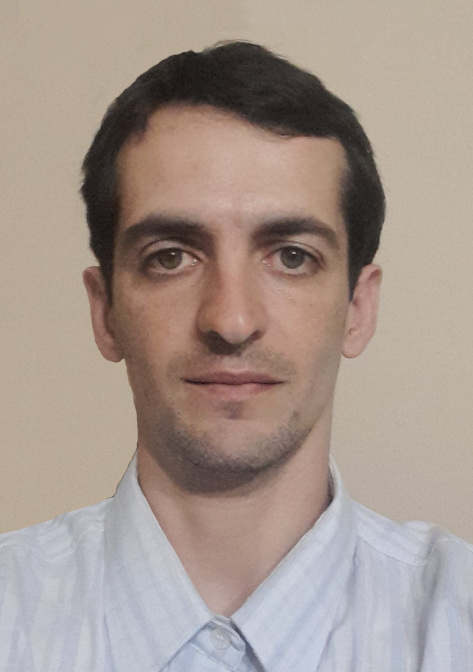
\includegraphics[width=3cm,clip=true]{cara1.jpg}}
\end{picture}\\
{\color{blue}\section*{Formación académica}}
\hrule
\begin{tabular}{l l}
  \multicolumn{1}{l}{\textbf{Secundario}}\\
  2006-2008&Polimodal: modalidad economía.\\
           &\small{Colegio Sagrado Corazón, Venado Tuerto.}\\
  \multicolumn{2}{l}{\textbf{Terciario}}\\
  2009-2017&Analista en computación administrativa.\\
           &\small{Instituto católico de enseñanza superior (ICES), Venado Tuerto.}\\
  \multicolumn{2}{l}{\textbf{Otros estudios}}\\
  2015&Curso: Experto universitario de seguridad de la información.\\
           &\small{Universidad Tecnológica Nacional (UTN).}\\
  2018&Diplomatura en programación Java.\\
           &\small{Universidad Tecnológica Nacional (UTN).}\\
  \multicolumn{2}{l}{\textbf{Estudios incompletos}}\\
  2012-2013&Licenciatura en ciencias de la computación.\\
           &\small{Facultad de ciencias exactas, ingeniería y agrimensura (FCEIA), Rosario.}\\
           &\small{Estado: 17 de 31 materias aprobadas.}\\
\end{tabular}\\
{\color{blue}\subsection*{Idiomas}}
\hrule
\begin{tabular}{l l}
  Inglés&Nivel intermedio/avanzado (B2).\\
\end{tabular}\\
{\color{blue}\subsection*{Experiencia laboral}}
\hrule
\begin{tabular}{l l}
  2014-2021&Cadetería Serpet.\\
  2021-Hoy&Cadetería particular.
\end{tabular}\\
{\color{blue}\subsection*{Otros datos de interés}}
\hrule
\begin{tabular}{l}
  Carné de conducir B-1.\\
\end{tabular}
\end{document}
